
\subsection{Elements}

Having concluded our survey of material and philosophical history, we are ready to develop the theory.
Our goal will be to develop a representation of subjective experience that is amenable to formal analysis.

Central to this theory will be the notion of pairwise preferences, which we have attempted to justify as a valid, yet formal, representation of subjective experience.

Before we can assess preference, we must establish some criterion to evaluate preferences against.
Among the same candidate set of answers, different questions can easily lead to different preferences.
For example, ranging over the items in your fridge, the questions \say{what to eat for breakfast} and \say{what to eat for dinner} will (likely) lead to different preferences among the same set of options.

\bigskip

We define questions with maximum generality, considering a general \say{question object} $Q$.
The representation of $Q$ is intentionally unspecified; the specific from of $Q$ will affect only the interpretation of the results, not the underlying theory.

We anticipate that $Q$ will often be represented via a string of characters (as in the fridge example).
However, $Q$ could be an image, a sound, an equation, or some new object yet unimagined.

\bigskip

In order to ask questions, we need candidate answers.
These candidate answers are members of an \textit{answer set} $A$.
As with the question object $Q$, the specific representation of the elements of $A$ are intentionally unspecified.

\bigskip

In order to represent subjective experience, we need an entity capable of subjective experience.
Discussions of subjectivity inevitably involve discussions of the notoriously elusive topic consciousness.
While the exact nature of consciousness is not known, researchers generally agree that conscious experience is attributed to discrete entities: as an entity I have an experience of consciousness that is separate from the experiences of other entities.
 
To resolve group preferences, we need a set of such discrete entities.
This set of entities is denoted $E$.
Unsurprisingly and in the spirit of this exposition, we leave the specific nature of these entities intentionally unspecified.
We anticipate that these entities will often be people. Later in this work we will introduce potential new directions for this theory, for which we may want to define these entities differently. Specifically, we will see how the problem of defining entities can be understood as selecting an \say{access policy}, the choice of which will shape the interpretation of the results.

\bigskip

Having introduced questions, answers, and entities, we are ready to introduce the \say{preference}, conceived of as a basic unit of subjective experience. As the name suggests, a preference represents an \textit{answer to a question}. Preferences have five components:

\begin{enumerate}
	\item A question object $Q$.
	\item An entity $e \in E$.
	\item A candidate answer $\alpha \in A$.
	\item A second candidate answer $\beta \in A$.
	\item The preference $p \in \{0, 1\}$, where $0$ corresponds to preferring $\alpha$.
\end{enumerate}

It is not immediately obvious how we might operate on this representation. Recalling that preferences are only defined relative to a question $Q$, we can make $Q$ implicit. Further, for the moment let us assume that we are interested only in the preferences of a single entity $e$.

Now, we see that the salient attributes of a preference are the two options $\alpha, \beta$, as well as the preference $p$. If we imagine $\alpha$ and $\beta$ as nodes, then $p$ can be represented as a directed edge between the two. Specifically, we create an edge $(\beta, \alpha)$ if $p = 0$ or $(\alpha, \beta)$ if $p = 1$ (the edge flows from loser to winner):

\begin{center}
\begin{tikzpicture}[node distance=3cm]
\node [roundnode] (a) {$\alpha$};
\node [roundnode] (b) [right of=a] {$\beta$};
\draw[ultra thick, <-] (a) -- (b);
\end{tikzpicture}
\end{center}

This graphical representation is desirable, as it suggests a natural way of aggregating preference. Imagine we have $A = \{a, b, c, d\}$, and an entity $e$ generates the following preferences:

\begin{center}
\socrata{a}{b}
\socrata{a}{c}

\socrata{b}{d}
\socrata{c}{b}

\end{center}

We can aggregate these preferences into the following \textit{preference graph} $S$:

\begin{center}
\begin{tikzpicture}[node distance=3cm]
\node [roundnode] (a) {a};
\node [roundnode] (b) [right of=a] {b};
\node [roundnode] (c) [below of=a] {c};
\node [roundnode] (d) [right of=c] {d};
\draw[ultra thick, ->] (b) -- (a);
\draw[ultra thick, ->] (c) -- (a);
\draw[ultra thick, ->] (d) -- (b);
\draw[ultra thick, ->] (b) -- (c);
\end{tikzpicture}
\end{center}

Aggregating preferences across multiple entities presents little difficulty.
If we have entity $\alpha$ generating the following (an ordered preference of $a, b, c$):

\begin{center}
\socrata{a}{b}
\socrata{a}{c}
\socrata{b}{c}
\end{center}

And entity $\beta$ generating the following (an ordered preference of $a, c, b$):

\begin{center}
\socrata{a}{b}
\socrata{a}{c}
\socrata{c}{b}
\end{center}


We can assign each preference a weight of 1 and combine the edges.
Parallel edges sum, while antiparallel edges cancel:

\begin{center}
\begin{tikzpicture}[node distance=3cm]
\node [roundnode] (a) {a};
\node [roundnode] (b) [right of=a] {b};
\node [roundnode] (c) [below of=a] {c};
\draw[ultra thick, ->] (b) to[bend right] node[below] {1} (a);
\draw[ultra thick, ->] (b) -- node[below] {1} (a);
\draw[ultra thick, ->] (c) to[bend right]  node[below] {1} (b);
\draw[ultra thick, ->] (b) -- node[below] {1} (c);
\draw[ultra thick, ->] (c) to[bend left]  node[left] {1} (a);
\draw[ultra thick, ->] (c) -- node[right] {1} (a);
\end{tikzpicture}
\hspace{5mm}
\raisebox{2 cm}{$\rightarrow$}
\hspace{5mm}
\begin{tikzpicture}[node distance=3cm]
\node [roundnode] (a) {a};
\node [roundnode] (b) [right of=a] {b};
\node [roundnode] (c) [below of=a] {c};
\draw[ultra thick, ->] (b) -- node[auto] {2} (a);
\draw[ultra thick, ->] (c) -- node[auto] {2} (a);
\end{tikzpicture}
\end{center}

It is instructive to see what occurs in the instance of two entities with opposing preferences.
Say we $\alpha$ with preferences $(a, b, c)$, and $\beta$ with preferences $(c, b, a)$.
We might say we could resolve this by selecting $b$, as this seems the mutually-agreeable option.

Is this principled?
Selecting $b$ would cause both entities to have their second preference, a forfeiting of one item each.
Selecting $a$ or $c$, on the other hand, would cause one entity to have its first preference, and the other third --- a forfeiture of two items.
In a sense, this pair of opposing preferences render all answers equal.

Observe what happens in the corresponding preference graph:

\begin{center}
\begin{tikzpicture}[node distance=3cm]
\node [roundnode] (a) {a};
\node [roundnode] (b) [right of=a] {b};
\node [roundnode] (c) [below of=a] {c};
\draw[ultra thick, ->] (b) to[bend right] node[below] {1} (a);
\draw[ultra thick, ->] (a) -- node[below] {1} (b);
\draw[ultra thick, ->] (c) to[bend right]  node[below] {1} (b);
\draw[ultra thick, ->] (b) -- node[below] {1} (c);
\draw[ultra thick, ->] (a) to[bend right]  node[right] {1} (c);
\draw[ultra thick, ->] (c) -- node[right] {1} (a);
\end{tikzpicture}
\hspace{5mm}
\raisebox{2 cm}{$\rightarrow$}
\hspace{5mm}
\begin{tikzpicture}[node distance=3cm]
\node [roundnode] (a) {a};
\node [roundnode] (b) [right of=a] {b};
\node [roundnode] (c) [below of=a] {c};
\end{tikzpicture}
\end{center}

The answers are disconnected; we interpret as an absence of preference.

\bigskip

\textit{A note on method:} we have been very intentional in our avoidance of assigning numerical value to subjective preference.
For an \textit{individual} entity (with an emphasis on the literal meaning of \say{individual} as non-divisible), preference is non-numeric.
Populations have magnitudes, however, and so we can comfortably reason in terms of sums and ratios when considering aggregations of entity preferences.

\subsection{A Probabilistic View}

Let us now consider some structural properties of preference graphs, and interpret them through the lens of preference resolution.
In this discussion, we will employ the elements of probabilistic methods of Paul \cite{erdos:1959}.

\bigskip

In the language of computer science, we denote graphs as $G = (V, E)$, with graph $G$ consisting of some set $V$ of \textit{vertices} (or \textit{nodes}) and some set $E$ of \textit{edges} between the vertices.
Edges can be directed or undirected, and are denoted $(u,v) \in E$, with $u, v \in V$.
When analyzing complexity, we use $n = |V|$, the number of vertices, and $m = |E|$, the number of edges.
We done the number of incoming edges for node $u$ as $in(u)$, and the number of outgoing edges as $out(u)$.
We refer to $in(u)$ as the ``indegree'' of $u$, and $out(u)$ as the ``outdegree'' of $u$.
Since an edge may exist between any pair of edges, we see that $m \leq n^2$.
In our case, there are ${n}\choose{2}$ possible pairs per graph.
Further, we see that $max_{u \in V}in(u) = n - 1$.

A vertex can be called a \textit{universal sink} if it has $in(u) = n - 1$.
In the context of preference, a universal sink is an option that is preferred over all others.
As a first pass, we can think of the problem of resolving preference as a problem of finding a universal sink, which can be found in O(n) time.

It might seem as the problem of preference resolution is simple: observe preferences, and find the universal sink.
Unfortunately, there is no guarantee that a universal sink will exist.

\bigskip

To show this, we will extend the $G(n,p)$ notation of Erd{\H o}s to the tournament graphs of \cite{landau:1953}.
A $G(n,p)$ graph is a random undirected graph of $n$ nodes, with the probability $p$ of an edge existing between any two nodes.
In this discussion, we will repurpose this notation to describe a different type of graph, a \textit{random tournament} $G_T(n,p)$, generated as follows:

\begin{enumerate}
	\item Create a complete graph of $n$ nodes.
	\item Remove all $(u,u)$ edges.
	\item Create a directed graph by randomly orienting the edges, with probability $p$ that $(u, v) \in E$ and probability $1-p$ that $(v, u) \in E$.
\end{enumerate}

We will show that as $n$ increases, the likelihood of a universal sink existing in a random tournament decreases exponentially.
Every vertex has $n-1$ edges.
For vertex $u$, to be a universal sink, all of these edges must point towards it.
If we consider a random tournament $G_T(n,p)$, then

\[
p(u_{usink}) = \prod_{v \in (V / \{u\})}p((u,v) \in E) = \frac{1}{2^{n-1}}
\]

Since the relationships between any pair of vertices is independent of all other pairs, the probability of \textit{any} sink is bounded by the sum of the probabilities of the individual vertices being sinks:

\[
p(G_{usink}) \leq \sum_{u \in V}p(u_{usink}) = \frac{n}{2^{n-1}}
\]

The likelihood of a universal sink existing in a random tournament decreases exponentially as $n$ increases.
If a tournament has no universal sink, then there must exist at least one \textit{cycle} in the tournament.
A cycle is a subset of vertices and edges such that there exists a \say{path} of edges such that any vertex in the cycle is reachable from any other.
Here is the simplest cycle between three vertices:

\begin{center}
\begin{tikzpicture}[node distance=3cm]
\node [roundnode] (a) {a};
\node [roundnode] (b) [right of=a] {b};
\node [roundnode] (c) [below of=a] {c};
\draw[ultra thick, <-] (a) -- (b);
\draw[ultra thick, <-] (b) -- (c);
\draw[ultra thick, <-] (c) -- (a);
\end{tikzpicture}
\end{center}

It is easy to see that this tournament has no universal sink.
From the perspective of preference, we interpret a cycle as a set of items which are preferred equally; alternatively, we can say that they are \textit{indistinguishable} from each other.

If there are $n$ vertices, then there are $n\choose{2}$ pairs.
Since there are two possible states for each pair, there are a total of $2^{n\choose{2}}$ possible graphs.
As an illustration, let's consider a triple, where $n = 3$.For every triple of vertices, there are $2^3 = 8$ possible permutations of edges:

\begin{center}
\begin{tikzpicture}[node distance=3cm]
\node [roundnode] (a) {a};
\node [roundnode] (b) [right of=a] {b};
\node [roundnode] (c) [below of=a] {c};
\draw[ultra thick, <-] (a) -- (b);
\draw[ultra thick, <-] (a) -- (c);
\draw[ultra thick, <-] (b) -- (c);
\end{tikzpicture}\quad
\begin{tikzpicture}[node distance=3cm]
\node [roundnode] (a) {a};
\node [roundnode] (b) [right of=a] {b};
\node [roundnode] (c) [below of=a] {c};
\draw[ultra thick, <-] (a) -- (b);
\draw[ultra thick, <-] (a) -- (c);
\draw[ultra thick, <-] (c) -- (b);
\end{tikzpicture} \quad
\begin{tikzpicture}[node distance=3cm]
\node [roundnode] (a) {a};
\node [roundnode] (b) [right of=a] {b};
\node [roundnode] (c) [below of=a] {c};
\draw[ultra thick, <-] (a) -- (b);
\draw[ultra thick, <-] (c) -- (a);
\draw[ultra thick, <-] (b) -- (c);
\end{tikzpicture}\vspace{5mm}
\begin{tikzpicture}[node distance=3cm]
\node [roundnode] (a) {a};
\node [roundnode] (b) [right of=a] {b};
\node [roundnode] (c) [below of=a] {c};
\draw[ultra thick, <-] (a) -- (b);
\draw[ultra thick, <-] (c) -- (a);
\draw[ultra thick, <-] (c) -- (b);
\end{tikzpicture} \quad
\begin{tikzpicture}[node distance=3cm]
\node [roundnode] (a) {a};
\node [roundnode] (b) [right of=a] {b};
\node [roundnode] (c) [below of=a] {c};
\draw[ultra thick, <-] (b) -- (a);
\draw[ultra thick, <-] (a) -- (c);
\draw[ultra thick, <-] (b) -- (c);
\end{tikzpicture}\quad
\begin{tikzpicture}[node distance=3cm]
\node [roundnode] (a) {a};
\node [roundnode] (b) [right of=a] {b};
\node [roundnode] (c) [below of=a] {c};
\draw[ultra thick, <-] (b) -- (a);
\draw[ultra thick, <-] (a) -- (c);
\draw[ultra thick, <-] (c) -- (b);
\end{tikzpicture} \vspace{5mm}
\begin{tikzpicture}[node distance=3cm]
\node [roundnode] (a) {a};
\node [roundnode] (b) [right of=a] {b};
\node [roundnode] (c) [below of=a] {c};
\draw[ultra thick, <-] (b) -- (a);
\draw[ultra thick, <-] (c) -- (a);
\draw[ultra thick, <-] (b) -- (c);
\end{tikzpicture}\quad
\begin{tikzpicture}[node distance=3cm]
\node [roundnode] (a) {a};
\node [roundnode] (b) [right of=a] {b};
\node [roundnode] (c) [below of=a] {c};
\draw[ultra thick, <-] (b) -- (a);
\draw[ultra thick, <-] (c) -- (a);
\draw[ultra thick, <-] (b) -- (c);
\end{tikzpicture}
\end{center}

In the case of three vertices, we see cycles in two out of eight possible graphs.
It is worth noting that while the absence of cycles in a random tournament necessarily implies the presence of a universal sink, the presence of a cycle does not necessarily imply the absence of a universal sink.
To see this, consider the following four-vertex directed graph:

\begin{center}
\begin{tikzpicture}[node distance=3cm]
\node [roundnode] (a) {a};
\node [roundnode] (b) [right of=a] {b};
\node [roundnode] (c) [below of=a] {c};
\node [roundnode] (d) [below of=b] {d};
\draw[ultra thick, <-] (a) -- (b);
\draw[ultra thick, <-] (a) -- (c);
\draw[ultra thick, <-] (a) -- (d);
\draw[ultra thick, <-] (b) -- (c);
\draw[ultra thick, <-] (c) -- (d);
\draw[ultra thick, <-] (d) -- (b);
\end{tikzpicture}
\end{center}

In this graph, vertices $\{c, b, d\}$ form a cycle, but $a$ is still a universal sink.
As discussed earlier, however, the likelihood of a universal sink existing in a random tournament, even allowing for cycles, decreases exponentially in $n$.

\bigskip

We raise this point to underscore that the presence of cycles does not imply the absence of meaningful structure; simply that meaningful structure will be more challenging to discern.
What is ``structure?''
American mathematician Claude Shannon defined a measure of structure, known as \textit{entropy}, which applied to probability distributions of random variables (\cite{cover}):

\[
H(X) = -\mathbb{E}[logp(X)] = -\sum_{x \in X}p(x)logp(x)
\]

Entropy is high when a distribution has a lot of uncertainty, and low when a distribution has little uncertainty.

This metric has proven invaluable: what analogous metrics might we develop for tournaments?
One possibility is the \textit{maximum indegree}, $max_{u \in V}in(u)$.
This metric can be calculated in $O(m + n)$ (linear time), and provides a rough sense of the amount of structure of the graph.

A second possibility is to look at the \textit{tournament entropy} $H_T$, the entropy of the empirical distribution of the indegrees of tournament $G$:

\[
H_T(G) = -\sum_{u \in V} \frac{in(u)}{m}log\bigg(\frac{in(u)}{m}\bigg)
\]

In the case of a three-node cycle, each node has an indegree of 1, equivalent to a uniform distribution over indegrees:

\begin{center}
\begin{tikzpicture}[node distance=3cm]
\node [roundnode] (a) {a};
\node [roundnode] (b) [right of=a] {b};
\node [roundnode] (c) [below of=a] {c};
\draw[ultra thick, ->] (b) -- (a);
\draw[ultra thick, ->] (c) -- (b);
\draw[ultra thick, ->] (a) -- (c);
\end{tikzpicture}
\hspace{5mm}
\raisebox{2 cm}{$\rightarrow$}
\hspace{5mm}
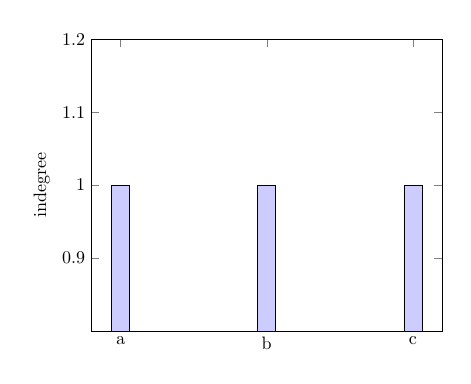
\begin{tikzpicture}[scale=0.65]
\begin{axis}[
    symbolic x coords={a, b, c},
    ylabel=indegree,
    xtick=data]
    \addplot[ybar,fill=white!80!blue] coordinates {
        (a,1)
        (b,1)
        (c,1)
    };
\end{axis}
\end{tikzpicture}
\end{center}

The tournament entropy of this graph is 1.585 bits, the maximum entropy distribution for three items.
In the case of a three-node transitive preference, we see a skewed distribution:

\begin{center}
\begin{tikzpicture}[node distance=3cm]
\node [roundnode] (a) {a};
\node [roundnode] (b) [right of=a] {b};
\node [roundnode] (c) [below of=a] {c};
\draw[ultra thick, ->] (b) -- (a);
\draw[ultra thick, ->] (c) -- (b);
\draw[ultra thick, ->] (c) -- (a);
\end{tikzpicture}
\hspace{5mm}
\raisebox{2 cm}{$\rightarrow$}
\hspace{5mm}
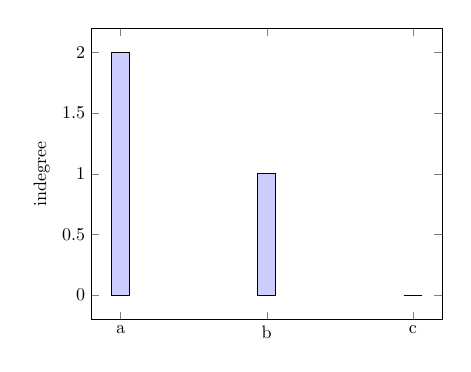
\begin{tikzpicture}[scale=0.65]
\begin{axis}[
    symbolic x coords={a, b, c},
    ylabel=indegree,
    xtick=data]
    \addplot[ybar,fill=white!80!blue] coordinates {
        (a,2)
        (b,1)
        (c,0)
    };
\end{axis}
\end{tikzpicture}
\end{center}

In this case, the tournament entropy is lower, only 0.918 bits.

\bigskip

We note that tournament entropy can be calculated in linear time.
Further, while this section has considered tournaments in which $m = {n\choose{2}}$ and every pair $\{u, v\}$ appears once, we can evaluate the tournament entropy of preference graphs with $m < {n\choose{2}}$ (graphs with partial observations), as well as thoughts with $m > {n\choose{2}}$ (graphs aggregating preferences of multiple entities).
When evaluating tournament entropy for preference graphs with large $m$, additional care must be taken as the distribution of observations across the pairs may not be uniform.

\subsection{A Linear Algebra View}

A graph can be represented as a matrix, with the values of the matrix corresponding to the values of the edges between nodes.
Let us denote the raw connection matrix as $C$.
By setting the values of the diagonal equal to the sum of their corresponding columns ($C_{ii} = \sum_j C_{ji}$), and normalizing the rows of this matrix ($\sum_i C_{ji} = 1$), we can construct a Markovian \say{transition matrix}, denoted $M$:

\begin{center}
\begin{minipage}{1.2in}
\begin{tikzpicture}[node distance=3cm]
\node [roundnode] (a) {a};
\node [roundnode] (b) [right of=a] {b};
\node [roundnode] (c) [below of=a] {c};
\draw[ultra thick, ->] (b) -- (a);
\draw[ultra thick, ->] (c) -- (b);
\draw[ultra thick, ->] (c) -- (a);
\end{tikzpicture}
\end{minipage}
\hfill
\begin{minipage}{1.2in}
\[
C=
  \begin{bmatrix}
    0 & 0 & 0 \\
    1 & 0 & 0 \\
    1 & 1 & 0
  \end{bmatrix}
\]
\end{minipage}
\hfill
\begin{minipage}{1.2in}
\[
M=
  \begin{bmatrix}
    1 & 0 & 0 \\
    .5 & .5 & 0 \\
    .5 & .5 & 0
  \end{bmatrix}
\]
\end{minipage}
\hfill
\end{center}



This matrix $M$ encodes the probability of ``transitioning'' from one item to another, with the values on the diagonal representing the likelihood of ``sticking with'' an item. 
If we imagine a vector $x_t \in \triangle^{V-1}$ representing the state at time $t$ as a distribution over all possible items, then

\[
x_{t+1} = x_t^TM
\]

gives us the distribution over items at time $t+1$.
If $M$ has certain properties (\textit{irreducible}, meaning that any item can be eventually reached from any other item, and \textit{aperiodic}, meaning that there are no stable loops among sets of states), then it can be shown that eventually $x$ will converge to a ``steady state'' distribution, in which $x = x^TM$ (\cite{lin:2016}).
Further, it can be shown that this steady state distribution, denoted $x_{\infty}$, is equivalent to the principal eigenvector of the matrix $M$, here denoted $v_1$.
The normalization of $M$ ensures that the principal eigenvector, denoted $\lambda_1$, is always equal to 1.

Interpreting $x_{\infty}$ as a distribution over items, then the components of $x_{\infty}$ with the largest values (probability) can be seen as the ``most preferred'' items.
The Perron-Frobenius theorem forms the foundation of these results, and use of this method has a long history (\cite{keener:1993}) and many applications, including the ranking of sports teams (\cite{landau:1915}) and websites (\cite{brin}).

\bigskip

It is worth discussing some interesting attributes of the principal eigenvector $v_1$.
First, by definition, $||v_1||_1$ (the $L_1$ norm) is equal to 1.
However, $||v_1||_2$ (the $L_2$ norm), varies.
Further, for $v_1$ with dimension $n$, $min(||v_1||_2^2) = n/n^2$, corresponding to a uniform preference over all items, and $max(||v_1||_2) = 1$, corresponding to a clear single preference.

\begin{proof}
As $||x||_2^2 \triangleq \sum x_i^2$, it will suffice to show that for any $\alpha \in \mathbb{R}, \epsilon > 0$,

\[
\bigg(\frac{1}{\alpha} + \epsilon\bigg)^2
+ \bigg(\frac{1}{\alpha} - \epsilon\bigg)^2
> \frac{2}{\alpha^2}.
\]

This is easily shown:

\[
\frac{1}{\alpha^2} + \frac{2\epsilon}{\alpha} + \epsilon^2
+ \frac{1}{\alpha^2} - \frac{2\epsilon}{\alpha} + \epsilon^2
 > \frac{2}{\alpha^2}
\]

\[
\frac{2}{\alpha^2} + 2\epsilon^2
 > \frac{2}{\alpha^2}
\]

\[
2\epsilon^2 > 0
\]
\end{proof}

This result suggests that $||v_1||_2$ can serve as an alternative measure of preference structure, with larger values implying more structured preference.
Further, for multiple entities, comparisons of entity-specific $v_1$ may be interpretable as comparisons of preference (entities with smaller distances between $v_1$ have more similar preferences, etc).
More work remains to be done understanding the specific behavior of $v_1$ and possible applications as a measure of preference structure beyond the standard application as a ranking.

\bigskip

With these concepts in hand, we can now ask what these steady states might look like for a series of simple preference graphs (Figures \ref{fig:linalg_1}, \ref{fig:linalg_2}, \ref{fig:linalg_3}, \ref{fig:linalg_4}, \ref{fig:linalg_5}, \ref{fig:linalg_6}).

% BEGIN LINALG FIGURES

\begin{figure}[!htb] % Two node transitive
\centering
\begin{minipage}{1.2in}
\begin{tikzpicture}[node distance=3cm]
\node [roundnode] (a) {a};
\node [roundnode] (b) [right of=a] {b};
\draw[ultra thick, ->] (b) -- (a);
\end{tikzpicture}
\end{minipage}
\hfill
\begin{minipage}{1.2in}
\[
M=
  \begin{bmatrix}
    1 & 0 \\
    1 & 0 \\
  \end{bmatrix}
\]
\end{minipage}
\hfill
\begin{minipage}{1.2in}
\begin{tikzpicture}
\def\v{2}
\def\x{2} % 2 * 1
\coordinate (O) at (0,0);
\coordinate (X) at (\x,0);
\draw [->] (O) -- (\v,0) node[below]{$x$};
\draw [->] (O) -- (0,\v) node[left]{$y$};
\draw [ultra thick, ->] (O) -- (X) node[right]{$v_1$};
\end{tikzpicture}
\end{minipage}
\caption{Preference graph $G$, transition matrix $M$, and principal eigenvector $v_1$ for a two-node transitive preference. $||v_1||_2^2 = 1$, $H_T(G) = 0$. Steady state achieved after one iteration.}
\label{fig:linalg_1} 
\end{figure}



\begin{figure}[!htb] % Two node cycle
\centering
\begin{minipage}{1.2in}
\begin{tikzpicture}[node distance=3cm]
\node [roundnode] (a) {a};
\node [roundnode] (b) [right of=a] {b};
\draw[ultra thick, ->] (b) to[bend right] (a);
\draw[ultra thick, ->] (a) to[bend right] (b);
\end{tikzpicture}
\end{minipage}
\hfill
\begin{minipage}{1.2in}
\[
M=
  \begin{bmatrix}
    .5 & .5 \\
    .5 & .5 \\
  \end{bmatrix}
\]
\end{minipage}
\hfill
\begin{minipage}{1.2in}
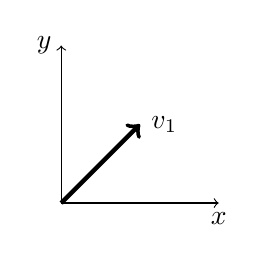
\begin{tikzpicture}
\def\v{2}
\def\x{1} % 2 * .5
\coordinate (O) at (0,0);
\coordinate (X) at (\x,\x);
\draw [->] (O) -- (\v,0) node[below]{$x$};
\draw [->] (O) -- (0,\v) node[left]{$y$};
\draw [ultra thick, ->] (O) -- (X) node[right]{$v_1$};
\end{tikzpicture}
\end{minipage}
\caption{Preference graph $G$, transition matrix $M$, and principal eigenvector $v_1$ for a two-node cycle. $||v_1||_2^2 = 1/2$, $H_T(G) = 1$. Intuitively, we set the probability of each item equal to the average of the prior preferences. The normalizing restriction on $v$ ensures that these averages continue to represent a distribution over the items. Note also that the steady state (a uniform distribution) is achieved after only one iteration.}
\label{fig:linalg_2} 
\end{figure}



\begin{figure}[!htb] % Three node transitive
\centering
\begin{minipage}{1.2in}
\begin{tikzpicture}[node distance=3cm]
\node [roundnode] (a) {a};
\node [roundnode] (b) [right of=a] {b};
\node [roundnode] (c) [below of=a] {c};
\draw[ultra thick, ->] (b) -- (a);
\draw[ultra thick, ->] (c) -- (b);
\draw[ultra thick, ->] (c) -- (a);
\end{tikzpicture}
\end{minipage}
\hfill
\begin{minipage}{1.2in}
\[
M=
  \begin{bmatrix}
    1 & 0 & 0 \\
    .5 & .5 & 0 \\
    .5 & .5 & 0
  \end{bmatrix}
\]
\end{minipage}
\hfill
\begin{minipage}{1.2in}
\begin{tikzpicture}
\def\v{2}
\def\x{2} % 2 * 1
\coordinate (O) at (0,0,0);
\coordinate (X) at (\x,0,0);
\draw [->] (O) -- (\v,0,0) node[below]{$x$};
\draw [->] (O) -- (0,\v,0) node[left]{$z$};
\draw [->] (O) -- (0,0,\v) node[below]{$y$};
\draw [ultra thick, ->] (O) -- (X) node[right]{$v_1$};
\end{tikzpicture}
\end{minipage}
\caption{Preference graph $G$, transition matrix $M$, and principal eigenvector $v_1$ for a three-node transitive preference. $||v_1||_2^2 = 1$, $H_T(G) = 0.918$. In this case, the steady state is achieved in the limit. At every iteration, C sends its probability mass to A and B evenly, and has no mass after the first iteration. B splits its mass between itself and A, while A directs all of its mass towards itself. The limiting convergence is due to the logarithmic reallocation of mass from B to A (a bit of a Zeno-style paradox).}
\label{fig:linalg_3} 
\end{figure}



\begin{figure}[!htb] % Three node cycle
\centering
\begin{minipage}{1.2in}
\begin{tikzpicture}[node distance=3cm]
\node [roundnode] (a) {a};
\node [roundnode] (b) [right of=a] {b};
\node [roundnode] (c) [below of=a] {c};
\draw[ultra thick, ->] (b) -- (a);
\draw[ultra thick, ->] (c) -- (b);
\draw[ultra thick, ->] (a) -- (c);
\end{tikzpicture}
\end{minipage}
\hfill
\begin{minipage}{1.2in}
\[
M=
  \begin{bmatrix}
    .5 & 0 & .5 \\
    .5 & .5 & 0 \\
    0 & .5 & .5
  \end{bmatrix}
\]
\end{minipage}
\hfill
\begin{minipage}{1.2in}
\begin{tikzpicture}
\def\v{2}
\def\x{.66} % 2 * 1/3
\coordinate (O) at (0,0,0);
\coordinate (X) at (\x,\x,\x);
\coordinate (Xxy) at (\x,0,\x);
\draw [->] (O) -- (\v,0,0) node[below]{$x$};
\draw [->] (O) -- (0,\v,0) node[left]{$z$};
\draw [->] (O) -- (0,0,\v) node[below]{$y$};
\draw [ultra thick, ->] (O) -- (X) node[right]{$v_1$};
\draw [dashed, color=red] (O) -- (Xxy);
\draw [dashed, color=red] (X) -- (Xxy);
\end{tikzpicture}
\end{minipage}
\caption{Preference graph $G$, transition matrix $M$, and principal eigenvector $v_1$ for a three-node cycle. $||v_1||_2^2 = 1/3$, $H_T(G) = 1.585$. Here the reallocation of probability mass across iterations exhibits more complex dynamics, and converges to $v_1$ in the limit.}
\label{fig:linalg_4} 
\end{figure}



\begin{figure}[!htb] % Three node double cycle
\centering
\begin{minipage}{1.2in}
\begin{tikzpicture}[node distance=3cm]
\node [roundnode] (a) {a};
\node [roundnode] (b) [right of=a] {b};
\node [roundnode] (c) [below of=a] {c};
\draw[ultra thick, ->] (b) to[bend right] (a);
\draw[ultra thick, ->] (c) to[bend right] (b);
\draw[ultra thick, ->] (a) to[bend right] (c);
\draw[ultra thick, ->] (a) -- (b);
\draw[ultra thick, ->] (b) -- (c);
\draw[ultra thick, ->] (c) -- (a);
\end{tikzpicture}
\end{minipage}
\hfill
\begin{minipage}{1.2in}
\[
M=
  \begin{bmatrix}
    .5 & .25 & .25 \\
    .25 & .5 & .25 \\
    .25 & .25 & .5
  \end{bmatrix}
\]
\end{minipage}
\hfill
\begin{minipage}{1.2in}
\begin{tikzpicture}
\def\v{2}
\def\x{.66} % 2 * 1/3
\coordinate (O) at (0,0,0);
\coordinate (X) at (\x,\x,\x);
\coordinate (Xxy) at (\x,0,\x);
\draw [->] (O) -- (\v,0,0) node[below]{$x$};
\draw [->] (O) -- (0,\v,0) node[left]{$z$};
\draw [->] (O) -- (0,0,\v) node[below]{$y$};
\draw [ultra thick, ->] (O) -- (X) node[right]{$v_1$};
\draw [dashed, color=red] (O) -- (Xxy);
\draw [dashed, color=red] (X) -- (Xxy);
\end{tikzpicture}
\end{minipage}
\caption{Preference graph $G$, transition matrix $M$, and principal eigenvector $v_1$ for a three-node double cycle. $||v_1||_2^2 = 1/3$, $H_T(G) = 1.585$}
\label{fig:linalg_5} 
\end{figure}



\begin{figure}[!htb] % Three node transitive with edge weights
\centering
\begin{minipage}{1.2in}
\begin{tikzpicture}[node distance=3cm]
\node [roundnode] (a) {a};
\node [roundnode] (b) [right of=a] {b};
\node [roundnode] (c) [below of=a] {c};
\draw[ultra thick, ->] (a) -- node[auto] {1} (b);
\draw[ultra thick, ->] (b) -- node[auto] {1} (c);
\draw[ultra thick, ->] (c) -- node[auto] {3} (a);
\end{tikzpicture}
\end{minipage}
\hfill
\begin{minipage}{1.2in}
\[
M=
  \begin{bmatrix}
    .75 & .25 & 0 \\
    0 & .5 & .5 \\
    .75 & 0 & .25
  \end{bmatrix}
\]
\end{minipage}
\hfill
\begin{minipage}{1.2in}
\begin{tikzpicture}
\def\v{2}
\def\a{1.09068489}
\def\b{0.54557228}
\def\c{0.36374283}
\coordinate (O) at (0,0,0);
\coordinate (X) at (\a,\c,\b);
\coordinate (Xxy) at (\a,0,\b);
\draw [->] (O) -- (\v,0,0) node[below]{$x$};
\draw [->] (O) -- (0,\v,0) node[left]{$z$};
\draw [->] (O) -- (0,0,\v) node[below]{$y$};
\draw [ultra thick, ->] (O) -- (X) node[right]{$v_1$};
\draw [dashed, color=red] (O) -- (Xxy);
\draw [dashed, color=red] (X) -- (Xxy);
\end{tikzpicture}
\end{minipage}
\caption{Preference graph $G$, transition matrix $M$, and principal eigenvector $v_1$ for a three-node cycle with edge weights. $||v_1||_2^2 = 0.4049$, $H_T(G) = 1.371$. Note how the introduction of variable weights repositions $v_1$ within the simplex, allowing us to recover a transitive ordering $a > b > c$.}
\label{fig:linalg_6} 
\end{figure}


\begin{figure}[!htb] % Four node two cycle
\centering
\begin{minipage}{1.2in}
\begin{tikzpicture}[node distance=3cm]
\node [roundnode] (a) {a};
\node [roundnode] (b) [right of=a] {b};
\node [roundnode] (c) [below of=a] {c};
\node [roundnode] (d) [below of=b] {d};
\draw[ultra thick, ->] (a) -- (c);
\draw[ultra thick, ->] (b) -- (a);
\draw[ultra thick, ->] (c) -- (b);
\draw[ultra thick, ->] (d) -- (a);
\draw[ultra thick, ->] (d) -- (b);
\draw[ultra thick, ->] (c) -- (d);
\end{tikzpicture}
\end{minipage}
\hfill
\begin{minipage}{1.2in}
\[
M=
  \begin{bmatrix}
    .66 & 0 & .33 & 0 \\
    .33 & .66 & 0 & 0 \\
    0 & .33 & .33 & .33 \\
    .33 & .33 & 0 & .33
  \end{bmatrix}
\]
\end{minipage}
\hfill
\begin{minipage}{1.2in}
\[
(.4, .3, .2, .1)
\]
\end{minipage}
\caption{Preference graph $G$, transition matrix $M$, and principal eigenvector $v_1$ for a four-node graph with two cycles. $||v_1||_2^2 = 0.3$, $H_T(G) = 1.918$.}
\label{fig:linalg_7} 
\end{figure}


\begin{figure}[!htb] % Four node upper cycle
\centering
\begin{minipage}{1.2in}
\begin{tikzpicture}[node distance=3cm]
\node [roundnode] (a) {a};
\node [roundnode] (b) [right of=a] {b};
\node [roundnode] (c) [below of=a] {c};
\node [roundnode] (d) [below of=b] {d};
\draw[ultra thick, ->] (a) -- (c);
\draw[ultra thick, ->] (c) -- (b);
\draw[ultra thick, ->] (b) -- (a);
\draw[ultra thick, ->] (d) -- (a);
\draw[ultra thick, ->] (d) -- (b);
\draw[ultra thick, ->] (d) -- (c);
\end{tikzpicture}
\end{minipage}
\hfill
\begin{minipage}{1.2in}
\[
M=
  \begin{bmatrix}
    .66 & 0 & .33 & 0 \\
    .33 & .66 & 0 & 0 \\
    0 & .33 & .66 & 0 \\
    .33 & .33 & .33 & 0
  \end{bmatrix}
\]
\end{minipage}
\hfill
\begin{minipage}{1.2in}
\[
(.33, .33, .33, 0)
\]
\end{minipage}
\caption{Preference graph $G$, transition matrix $M$, and principal eigenvector $v_1$ for a four-node graph with one cycle. $||v_1||_2^2 = 1/3$, $H_T(G) = 1.585$. Note that we see a cycle in $v_1$, despite having a larger $L_2$ value than the previous example.}
\label{fig:linalg_8} 
\end{figure}


\begin{figure}[!htb] % Four node lower cycle
\centering
\begin{minipage}{1.2in}
\begin{tikzpicture}[node distance=3cm]
\node [roundnode] (a) {a};
\node [roundnode] (b) [right of=a] {b};
\node [roundnode] (c) [below of=a] {c};
\node [roundnode] (d) [below of=b] {d};
\draw[ultra thick, ->] (b) -- (a);
\draw[ultra thick, ->] (c) -- (a);
\draw[ultra thick, ->] (d) -- (a);
\draw[ultra thick, ->] (b) -- (c);
\draw[ultra thick, ->] (c) -- (d);
\draw[ultra thick, ->] (d) -- (b);
\end{tikzpicture}
\end{minipage}
\hfill
\begin{minipage}{1.2in}
\[
M=
  \begin{bmatrix}
    1 & 0 & 0 & 0 \\
    .33 & .33 & .33 & 0 \\
    .33 & 0 & .33 & .33 \\
    .33 & .33 & 0 & .33
  \end{bmatrix}
\]
\end{minipage}
\hfill
\begin{minipage}{1.2in}
\[
(1, 0, 0, 0)
\]
\end{minipage}
\caption{Preference graph $G$, transition matrix $M$, and principal eigenvector $v_1$ for a four-node graph with one cycle. $||v_1||_2^2 = 1$, $H_T(G) = 1.793$. Note how the presence of a cycle in the lower nodes does not prevent the graph from having high level of structure.}
\label{fig:linalg_9} 
\end{figure}

% END LINALG FIGURES

This series of basic examples illustrate how the language of graphs and matrices allows us to make meaningful statements about preference in the presence of challenging structures like cycles, which manifest as contradictions when represented in terms of linear ordering.

\FloatBarrier

\subsection{Connections to Social Choice Theory}

Those readers familiar with the economics literature will see many parallels to the Social Choice Theory presented in \cite{arrow}.
In this work, Arrow proposed three criteria for good voting systems, and went on to famously prove that no voting system could exist which satisfied all three.
These criteria are:

\begin{itemize}
	\item \textbf{Unanimity}: if all voters prefer a to b, the group prefers a to b.
	\item \textbf{Non-dictatorship}: there is no individual voter whose preferences always prevail.
	\item \textbf{Independent of Irrelevant Alternatives (IIA)}: the group preference between a and b should be determined only by individual preferences between a and b (and not, for example, c).
\end{itemize}

Arrows impossibility theorem shows that these three criteria taken together can lead to contradiction.
We will give a sketch of the proof here (inspired by \cite{geanakoplos:2005}), as well as reinterpret the contradiction through the framework of preference graphs.

\bigskip

First, imagine we have a set $V$ of $N$ voters, asked to each submit a linear ordering of three items: $a, b$, and $c$.
The voters are partitioned into three sets as follows: $S_1 = \{V_1, ..., V_{k-1}\}$, $K = \{V_k\}$, and $S_2 = \{v_{k+1}, ..., V_N\}$, and all voters in each set always vote the same way.
Set $K$ consists of one voter, $V_k$, who we will refer to as the ``pivotal voter'' in that if $V_k$ votes the same way as either $S_1$ or $S_2$, then that preference prevails for the group.
In Figure \ref{fig:impossiblity_tables}, we see a sequence of three states of preference.
A contradiction emerges in the third state, when the preference reversals of $S_1$ and $S_2$ have no impact on the group preference.

\begin{figure}[!htb]
\centering
\begin{tabular}{ c | c | c | c }
 $S_1$ & $K$ & $S_2$ & Group \\ 
 \hline
 b & a & a & a \\ 
 c & b & b & b \\  
 a & c & c & c
\end{tabular}
 $\rightarrow$
\begin{tabular}{ c | c | c | c }
 $S_1$ & $K$ & $S_2$ & Group \\ 
 \hline
 b & \textbf{b} & a & \textbf{b} \\ 
 c & \textbf{a} & b & \textbf{a} \\  
 a & c & c & c
\end{tabular}
 $\rightarrow$
\begin{tabular}{ c | c | c | c }
 $S_1$ & $K$ & $S_2$ & Group \\ 
 \hline
 \textbf{c} & b & a & b \\ 
 \textbf{b} & a & \textbf{c} & a \\  
 a & c & \textbf{b} & c
\end{tabular}
\caption{Sequence of preference orderings for voter subsets $S_1$, $K$, and $S_2$, and final group preference. $V_k$ is a dictator in that the group prefers $b > c$ even though both $S_1$ and $S_2$ prefer $c > b$.}
\label{fig:impossiblity_tables} 
\end{figure}

In Figure \ref{fig:impossiblity_graphs}, we see the same sequence of preferences represented graphically.
In this view, we see that the ``paradox'' is simply the inability to represent cyclical preference as a linear ordering.
We also see how the IIA assumption becomes problematic, as the ordering of $b > a$ and $a > c$ inhibits the group ordering of $c > b$.
If we relax the IIA assumption and allow cycles, we see that the final preference graph of this proof has the same structure as our example graph in Figure \ref{fig:linalg_6}, and therefore has a steady state distribution of $c > a > b$.
Note that the eigenvector-based methods described earlier imply IIA relaxation.

\begin{figure}[!htb]
\centering
\begin{tikzpicture}[node distance=3cm]
\node [roundnode] (a) {a};
\node [roundnode] (b) [right of=a] {b};
\node [roundnode] (c) [below of=a] {c};
\draw[ultra thick, <-] (a) -- node[auto] {1} (b);
\draw[ultra thick, <-] (a) -- node[auto] {1} (c);
\draw[ultra thick, <-] (b) -- node[auto] {5} (c);
\end{tikzpicture}\quad
\begin{tikzpicture}[node distance=3cm]
\node [roundnode] (a) {a};
\node [roundnode] (b) [right of=a] {b};
\node [roundnode] (c) [below of=a] {c};
\draw[ultra thick, <-] (b) -- node[auto] {1} (a);
\draw[ultra thick, <-] (a) -- node[auto] {1} (c);
\draw[ultra thick, <-] (b) -- node[auto] {5} (c);
\end{tikzpicture} \quad
\begin{tikzpicture}[node distance=3cm]
\node [roundnode] (a) {a};
\node [roundnode] (b) [right of=a] {b};
\node [roundnode] (c) [below of=a] {c};
\draw[ultra thick, <-] (b) -- node[auto] {1} (a);
\draw[ultra thick, <-] (a) -- node[auto] {1} (c);
\draw[ultra thick, <-] (c) -- node[auto] {3} (b);
\end{tikzpicture}
\caption{Same sequence of preference orderings, shown as preference graphs. We set $|S_1| = |S_2| = 2$. $S_1$ and $S_2$'s reversal of preference between $b$ and $c$ in the third graph creates a cycle.}
\label{fig:impossiblity_graphs} 
\end{figure}

Here we see how the language of preference graphs clarifies the dynamics involved in social choice.
